%=============================================================================
% IMPLEMENTATION

\documentclass[../mpaper.tex]{subfiles}
\begin{document}

Similar to the situation described in \autoref{sec:Design} about selecting the right tools, we chose DX-focused tools, that integrate into an ecosystem, to develop the DX-based project. % The dashboard, called "\textit{Code Fitness}", was implemented over \href{https://github.com/ineshbose/code-fitness}{a public repository on GitHub}; see \autoref{fig:dashboard_interface} for the final product.

\subsubsection*{The Editor} % {Visual Studio Code}

We're aware of the popularity and extensibility of the Visual Studio Code (VSCode) text editor; we created an extension that can be enabled within the editor to provide the dashboard within the interface. Since VSCode is based on the Electron framework, which renders Chromium browser instances, and is written in TypeScript, extensions would also need to be based on Node.js. Moreover, VSCode provides several APIs that can enable functionality for its extensions; the Webview API\noteurl{https://code.visualstudio.com/api/extension-guides/webview} allowed the extension to embed our interface into the editor similar to an \texttt{iframe}. The environment could not be assumed to be the same as a traditional web browser as VSCode resources are local and specific to the users' computers, so we needed to consider all restrictions. Our webview gets registered after VSCode calls the exported \texttt{activate} function, can be launched from its Command Palette and renders on the main panel that is used to view \& edit code to take advantage of the large display with tabbed headings in groups. The extension was also \href{https://marketplace.visualstudio.com/items?itemName=2504266b-student-gla-ac-uk.code-fitness}{published and listed on the Visual Studio Marketplace}.

\subsubsection*{The Interface} % {SvelteKit \& Chart.js}

While we were able to create a Visual Studio Code extension, the interface had to be developed separately; this would be similar to creating webpages with HTML, CSS \& JavaScript. We chose to use SvelteKit\noteurl{https://kit.svelte.dev/}, to develop the interface, which is a modern web framework based on Svelte \& Vite\optionalnote{https://vitejs.dev/} (so DX was incredible) providing high performance \& compilation with static site generation (SSG) enabled. Serving our compiled application through Visual Studio Code was a difficult task, as VSCode expects HTML templates to be provided as a string, but we developed a custom bundler, using HTML parsers and JavaScript code generators, to enable the integration and keep the UI easy to maintain.

Finally, the interface must provide visualisations as that is the core purpose of our dashboard, but generating graphs on websites requires \texttt{canvas} elements and complex JavaScript code that needs to handle input of unknown type. This step was crucial to ensure the modular architecture of our system, and we chose to use the Chart.js\noteurl{https://www.chartjs.org/} library. It is the most popular JavaScript charting library (after D3.js) that can render different charts with great performance, responsiveness and customisation. The required input to generate a graph is a JSON object for which our system declared a consistent schema to be used in plugins.

The final product interface with generated graphs can be seen in \autoref{fig:dashboard_interface}. Component styles remained consistent with VSCode with the help of the Webview UI Toolkit\noteurl{https://github.com/microsoft/vscode-webview-ui-toolkit}.

\begin{figure}
    \centering
    % \begin{subfigure}{0.48\textwidth}
    %     \centering
    %     \frame{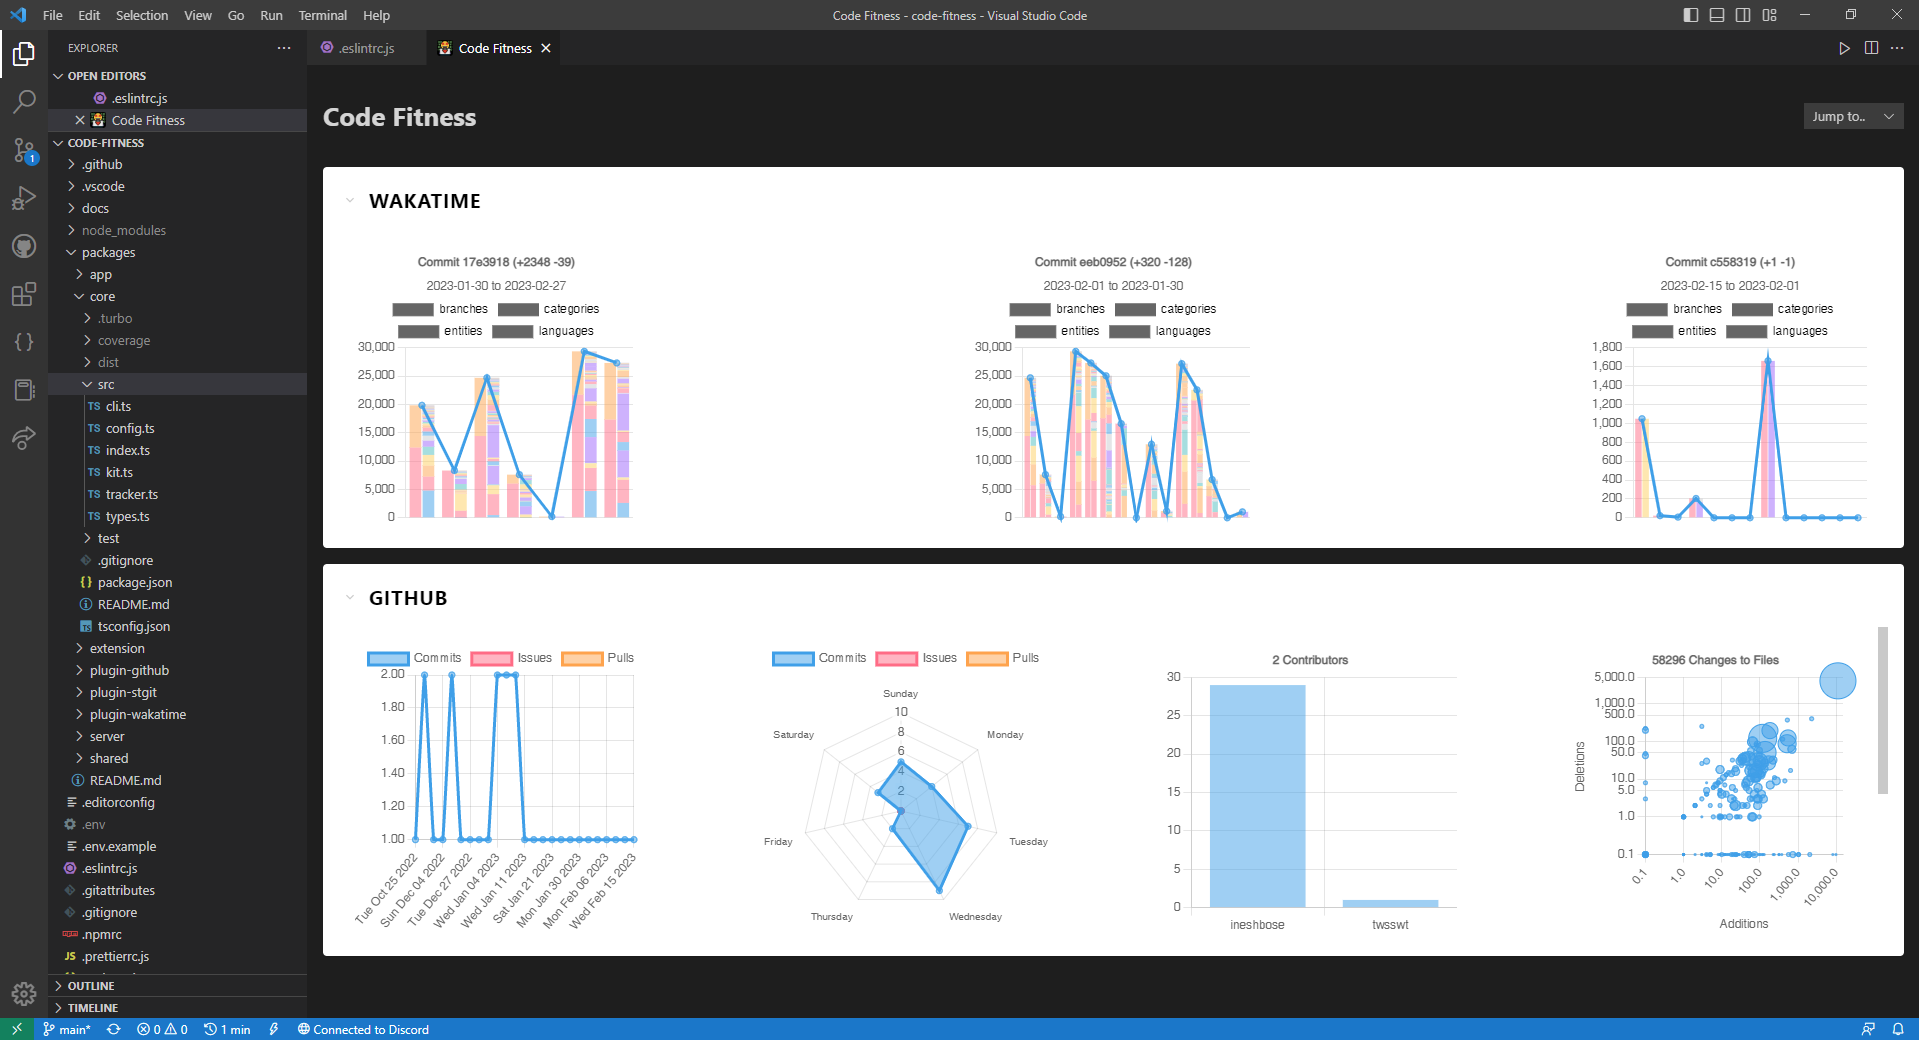
\includegraphics[width=\textwidth]{screenshot_27-02.png}}
    % \end{subfigure}
    % \vskip\baselineskip
    \begin{subfigure}{0.48\textwidth}
        \centering
        \frame{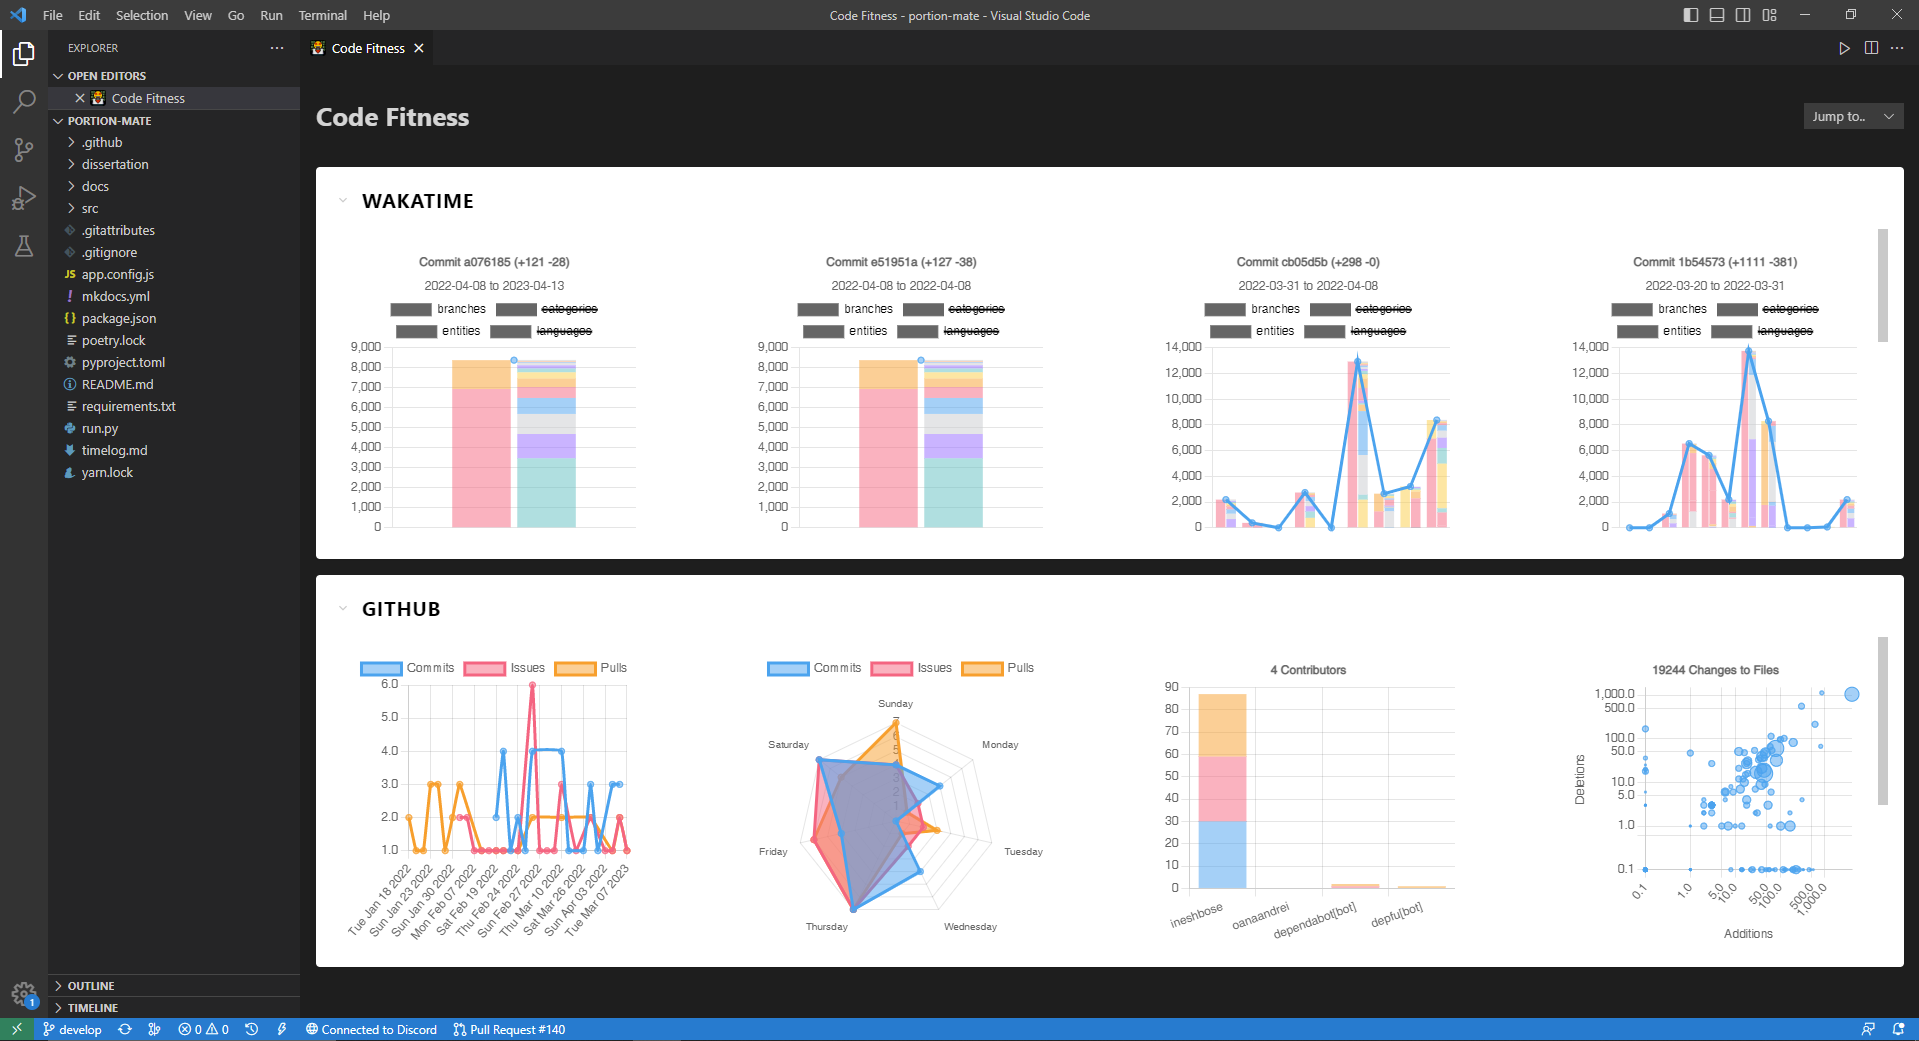
\includegraphics[width=\textwidth]{Screenshot_13-04-dark.png}}
    \end{subfigure}
    \vskip\baselineskip % \hfill
    \begin{subfigure}{0.48\textwidth}
        \centering
        \frame{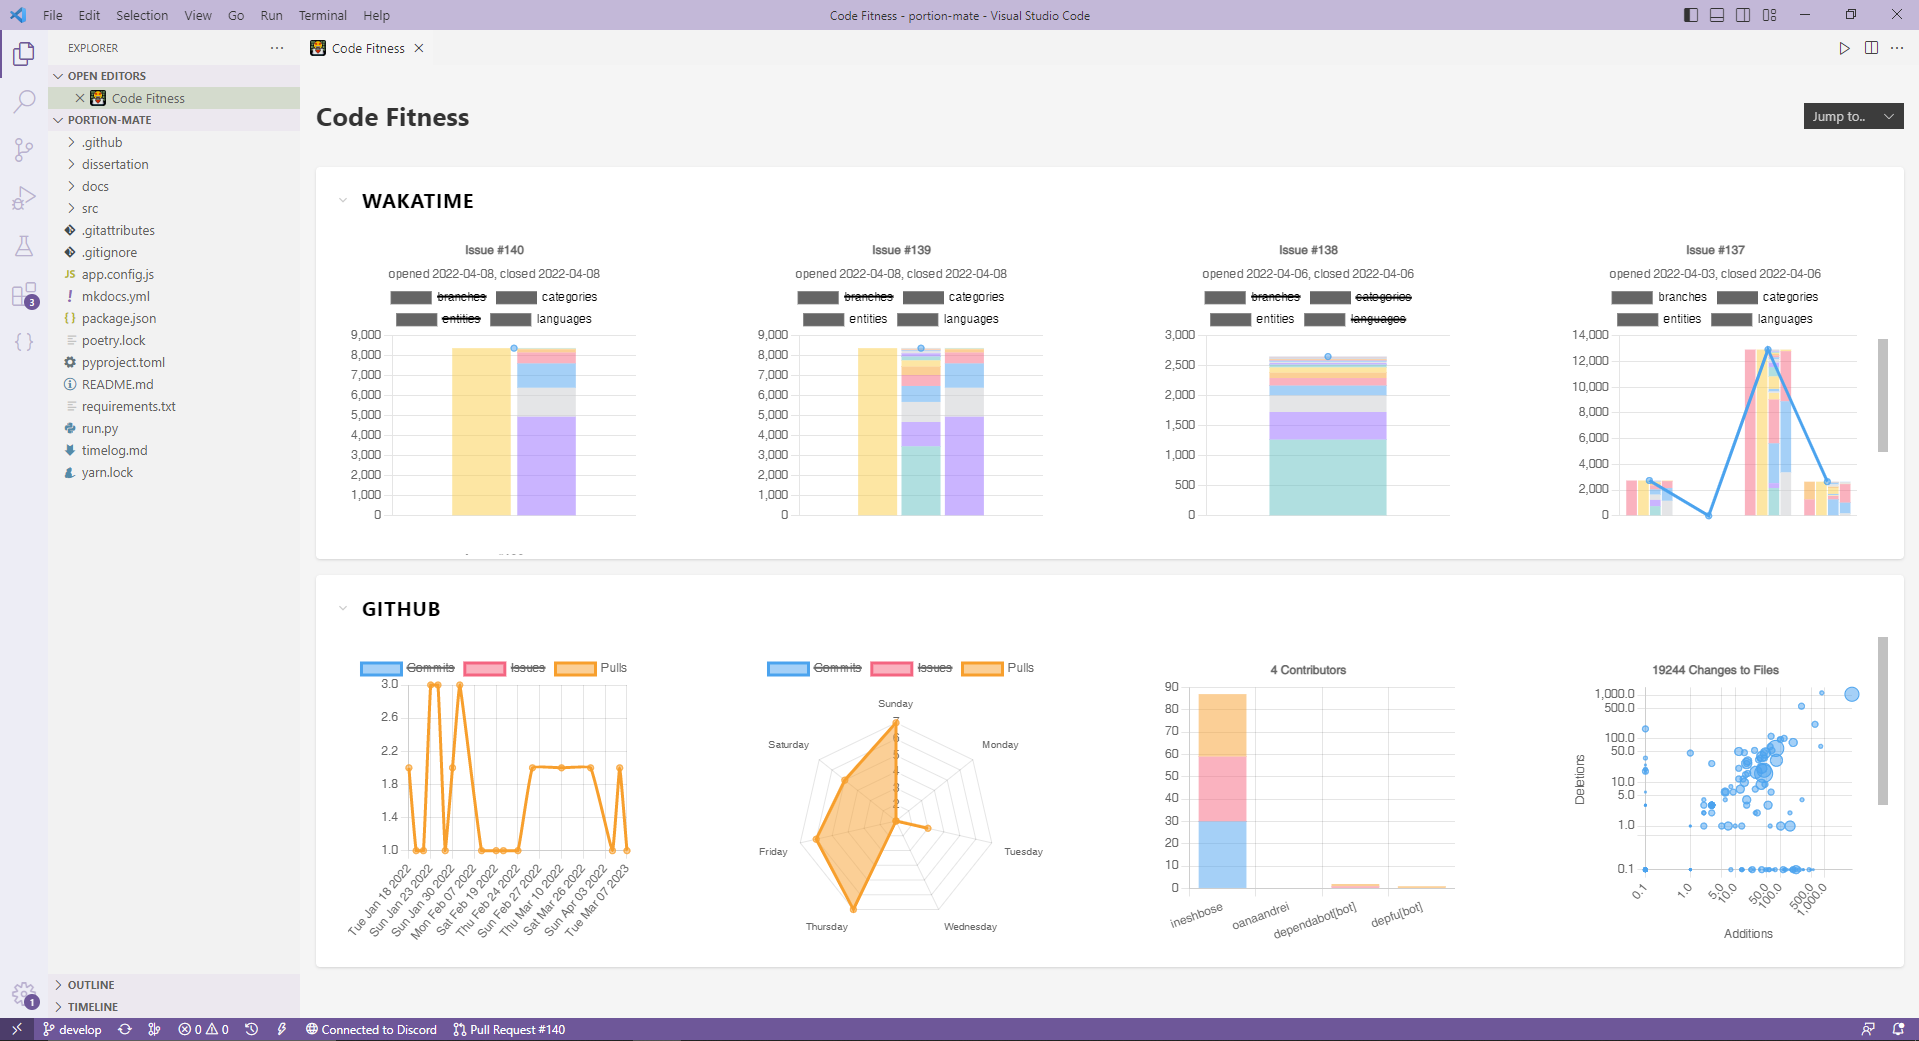
\includegraphics[width=\textwidth]{Screenshot_13-04-light.png}}
    \end{subfigure}
    % \vskip\baselineskip
    \caption{Dashboard Interface}
    \label{fig:dashboard_interface}
\end{figure}

\subsubsection*{Modular Architecture}

Using the core technologies mentioned above, we were able to setup our targeted modular architecture that could enable multiple visualisations to be generated from different sources without making changes to the extension or the interface. Since the repository uses the monorepo development strategy, each aspect of the system is abstracted into its own package, and integrated with the help of Turborepo and Yarn Workspaces. The \texttt{core} package implemented the logic of taking the configuration as input and loading it to process data from the plugins. Plugins are higher-order functions or objects with a \texttt{setup} function that provide access to APIs and return an \texttt{export} function back to be called by the loader; these can take declare required inputs from the configuration (such as endpoint URL, filter queries, and API token) and also take the loader context as input to get environment details and/or interact with other plugins; these functions can also be asynchronous with all \texttt{export} functions being executed concurrently. Since the project used TypeScript to ensure strong type-safety all-around the code, plugins take advantage of kit-utilities (such as \texttt{definePlugin}) exported by the core package to confirm that parameters and return values follow the schema. This architecture is heavily inspired by the Nuxt\noteurl{https://github.com/nuxt/nuxt} framework.

The \texttt{extension} package uses the SvelteKit app that calls the loader with the configuration -- it plugs into the extension (see \autoref{fig:system_architecture}) through the exported \texttt{webview} function generated by the custom builder. This custom builder mediates the Vite SSG template with hashed URLs for static assets so that the VSCode Webview can render properly with the \texttt{vscode://} protocol. This means that the extension is also designed to be framework-agnostic, i.e. it is not specific to our interface built through SvelteKit, but can be redeveloped in other front-end frameworks like React \& Angular. In addition to the cyclic, asynchronous flow of control between the plugins \& APIs in the core package (see \autoref{fig:user_flow}), VSCode itself provides APIs and modularity through extensions, so our implementation also uses other VSCode extensions' utilities to generate data - like \texttt{vscode.git} to safely get remote URL, and \texttt{GitHub.vscode-pull-request-github} to automatically register API token. The \href{https://github.com/ineshbose/code-fitness/blob/f5630aaea7eb129770a42115677da1d326ebd309/packages/extension/package.json#L18-L56}{\texttt{package.json}} showcases usage of internal packages and configuration for VSCode through the "\texttt{contributes}" field.

\subsubsection*{Initial Plugins}

As the plugins in the system provide Chart.js schema data for the visualisations, it would need to be generated from appropriate sources such as their repository (such as commits, issues), their IDE (keystrokes, build status) and their browser (websites, active tab). We developed plugins for GitHub as it is the most popular hosting platform and it provides a powerful API with detailed documentation. Some constraints were introduced due to the API requiring authentication and rate-limits; in most cases, we were able to adjust our design to be compliant and efficient.

The main plugin was for WakaTime\noteurl{https://wakatime.com/}. It is a software productivity analytics service that collects and displays developers' coding activities through a range of integrations and plugins for popular development environments, including VSCode \& Google Chrome, along with an API. This was extremely useful to the project as it removed massive complexities required for our system and our implementation would only need to map the data from the WakaTime API to the repository data generating suitable, intuitive graphs.

\begin{figure*}[ht]
    \centering
    \begin{subfigure}{\textwidth}
        \centering
        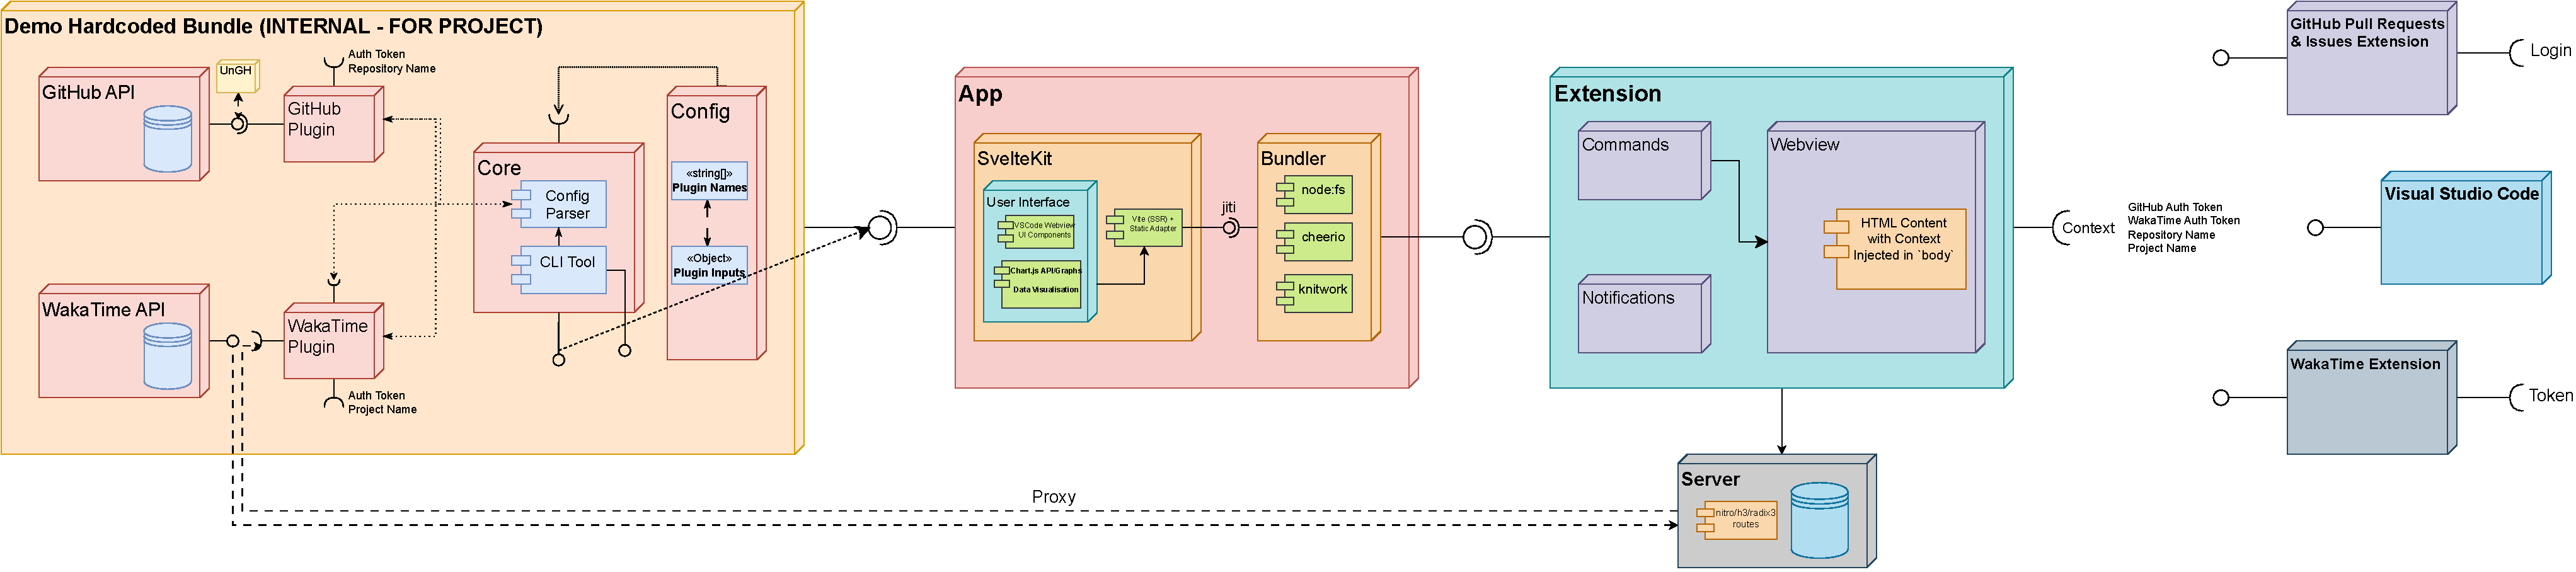
\includegraphics[width=0.95\textwidth]{architecture-wide.pdf}
        \caption{Modular architecture of the system}
        \label{fig:system_architecture}
    \end{subfigure}
    \vskip\baselineskip
    \begin{subfigure}{\textwidth}
        \centering
        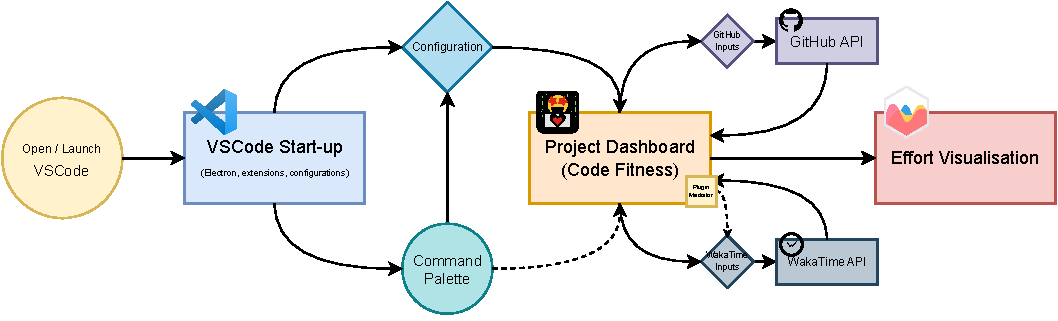
\includegraphics[width=0.75\textwidth]{simplified-flow.pdf}
        \caption{Simplified user flow for using the dashboard}
        \label{fig:user_flow}
    \end{subfigure}
    \caption{Infrastructure for the implementation}
\end{figure*}

\end{document}
